% CECI EST UN FICHIER DE MODÈLE LATEX POUR LES ARTICLES INCLUS DANS
% *Anthology of Computers and the Humanities*. AJOUTEZ L’OPTION
% 'final' LORS DE LA CRÉATION DE LA VERSION FINALE DE L’ARTICLE. 
% NE PAS modifier la classe du document
\documentclass[final,fra]{anthology-ch} % pour la version finale
%\documentclass[fra]{anthology-ch}         % pour la soumission

% CHARGER LES PACKAGES LaTeX
\usepackage{booktabs}
\usepackage{graphicx}
\usepackage{xcolor}
\usepackage{enumitem}
\usepackage{pifont}
\usepackage{csquotes}
\usepackage{pifont}
\usepackage{float}
\usepackage{subcaption}

\definecolor{deepblue}{RGB}{0, 0, 180}
\newcommand{\Gon}[1]{\textcolor{deepblue}{#1}}

% TITRE DE LA SOUMISSION
\title{Les formats d'encodage de la notation musicale à l'épreuve d'un objectif de transcription manuscrite automatique} 

% INFORMATIONS SUR LES AUTEURS ET LES AFFILIATIONS
\author[1]{Hugo Scheithauer}[
  orcid=https://orcid.org/0000-0002-5659-4675,
  email=hugo.scheithauer@inria.fr
]

\author[2]{Gonzalo Romero-García}[
  orcid=0000-0003-1971-6204,
  email=gonzalo.romero-garcia@epita.fr
]

\author[1]{Laurent Romary}[
  orcid=0000-0002-0756-0508,
  email=laurent.romary@inria.fr
]

\author[1]{Thibault Clérice}[
  orcid=0000-0003-1852-9204,
  email=thibault.clerice@inria.fr
]

\affiliation{1}{Inria, ALMAnaCH, Paris, France}
\affiliation{2}{EPITA Research Laboratory, Image Processing and Pattern Recognition, Paris, France}


% MOTS-CLÉS
\keywords[fra]{reconnaissance optique de musique, transcription automatique de partitions manuscrites, transcription, jeu de données, standards, notation musicale occidentale}
\keywords[eng]{optical music recognition, handwritten music recognition, transcription, dataset, standards, common western music notation}

% MÉTADONNÉES DE LA PUBLICATION (par défaut pour le moment)
\pubyear{2026}
\pubvolume{4}
\pagestart{108}
\pageend{119}
\paperorder{15}
\conferencename{Actes de la Conférence Humanistica}
\conferenceeditors{Serena Crespi, Simon Gabay, Martin Grandjean, Ariane Pinche, Marie Puren et Léa Saint-Raymond}
\doi{10.63744/K2fvu4Nzsv6t}
\customhead{}

\addbibresource{bibliography.bib}

%%%%%%%%%%%%%%%%%%%%%%%%%%%%%%%%%%%%%%%%%%%%%%%%%%%%%%%%%%%%%%%%%%%%%%%%%%%
% DÉBUT DU TEXTE
\begin{document}

%TC:ignore
\maketitle

\begin{abstract}
Le développement de la reconnaissance automatique de partitions (\textit{Optical Music Recognition}, OMR) se heurte à une fragmentation des formats de représentation, répartie entre exigences éditoriales (MEI), impératifs de rendu graphique et de sémantique (MusicXML) et analyse computationnelle (Humdrum **kern). Cette tension est particulièrement saillante pour les sources manuscrites, où la sémantique musicale se double d'une matérialité documentaire complexe. S'appuyant sur les récents progrès de l'ATR (Automatic Text Recognition), cet article évalue la capacité des standards actuels à servir de vérités de terrain. En prenant pour cas d'étude les manuscrits de piano de Claude Debussy, nous défendons une approche graphématique de la transcription. Nous justifions le détournement de MusicXML vers un modèle \enquote{structurel} capable de préserver, dans une certaine mesure, l'ancrage physique et les phénomènes non-standards de la source. Cette proposition vise à participer à la stabilisation des pratiques d'annotation pour la création de jeux de données mutualisables, condition essentielle au développement d'un OMR historique robuste.
\end{abstract}
%TC:endignore

\section{Introduction}

Le développement des technologies de transcription automatique de texte (ou \textit{Automatic Text Recognition}, ATR) a permis d'ouvrir de nouvelles voies d'accès à grande échelle pour les documents textuels, fruit d'un effort collectif de la communauté scientifique. Si les bibliothèques numériques offrent aujourd'hui un accès massif au patrimoine textuel, le patrimoine musical écrit n'est pas en reste. À titre d'exemple, la plateforme de la Bibliothèque nationale de France (BnF), Gallica\footnote{Voir le site internet de \href{https://gallica.bnf.fr/accueil/fr/html/accueil-fr}{Gallica}. Consulté le 12/01/26.}, héberge un corpus de 76 105 documents rassemblés sous l’appellation \enquote{partitions}, qu'il s'agisse de pièces uniques ou de recueils.  

Le pendant de l'ATR pour la notation musicale est l'\textit{Optical Music Recognition} (OMR). Cette tâche regroupe les méthodes visant à transformer automatiquement une image de partition imprimée ou manuscrite en une représentation exploitable par une machine. L'OMR se confronte à de nombreux défis inhérents à la nature de la notation musicale \cite{castellanos_deep_2025}~: la non-linéarité de la notation, la superposition et les relations entre symboles, la richesse du vocabulaire et l'imbrication possible entre notation musicale et texte. 

Par conséquent, les formats de représentation divergent naturellement de ceux utilisés pour le texte. L'encodage de la notation musicale est marqué par une tension entre trois approches : la représentation des documents, portée par des systèmes favorisés par la musicologie et les humanités en général comme le format XML de la \textit{Music Encoding Initiative} (MEI)~\cite{music_encoding_initiative_mei_2025}~; des systèmes de représentation de la musique pour la partager et à destination des personnes qui la jouent avec MusicXML~\cite{good_musicxml_2001}~; et des représentations fonctionnelles de la seule sémantique musicale avec le format Humdrum **kern~\cite{huron_music_2002}, destiné à l'analyse musicologique computationnelle. Cette division entre formats et objectifs de représentation illustre l'opposition entre données d'usage et données d'entraînement, et les standards actuels, hérités de l'édition ou de la musicologie computationnelle, peinent à concilier précision documentaire, description graphique et validité musicale.

Après un état de l'art sur l'encodage de la musique et les corpus destinés à l'OMR, nous évaluerons d'abord la capacité des trois principaux formats cités précédemment à servir de vérité de terrain. Nous justifierons ensuite le choix de MusicXML comme compromis opérationnel, en précisant les limites inhérentes à ce format lorsqu'il est employé dans une transcription graphématique de source manuscrite. 

Nos contributions sont les suivantes : 

\begin{itemize}
    \item \textbf{Évaluation critique des formats d'encodage} : une analyse comparative des formats MEI, MusicXML et Humdrum **kern sous l'angle spécifique de la production de données d'entraînement pour l'OMR de partitions manuscrites.
    \item \textbf{Justification méthodologique de MusicXML} : la démonstration du potentiel de MusicXML comme standard de compromis pour décrire une source manuscrite dans le contexte de l'OMR.
    \item \textbf{Ouverture vers l'OMR « de source »} : une proposition de changement de paradigme, passant de la seule reconnaissance du contenu sémantique musical à une transcription respectant la dimension documentaire et l'hétérogénéité des manuscrits.
\end{itemize}

\begin{figure}[H]
    \centering
    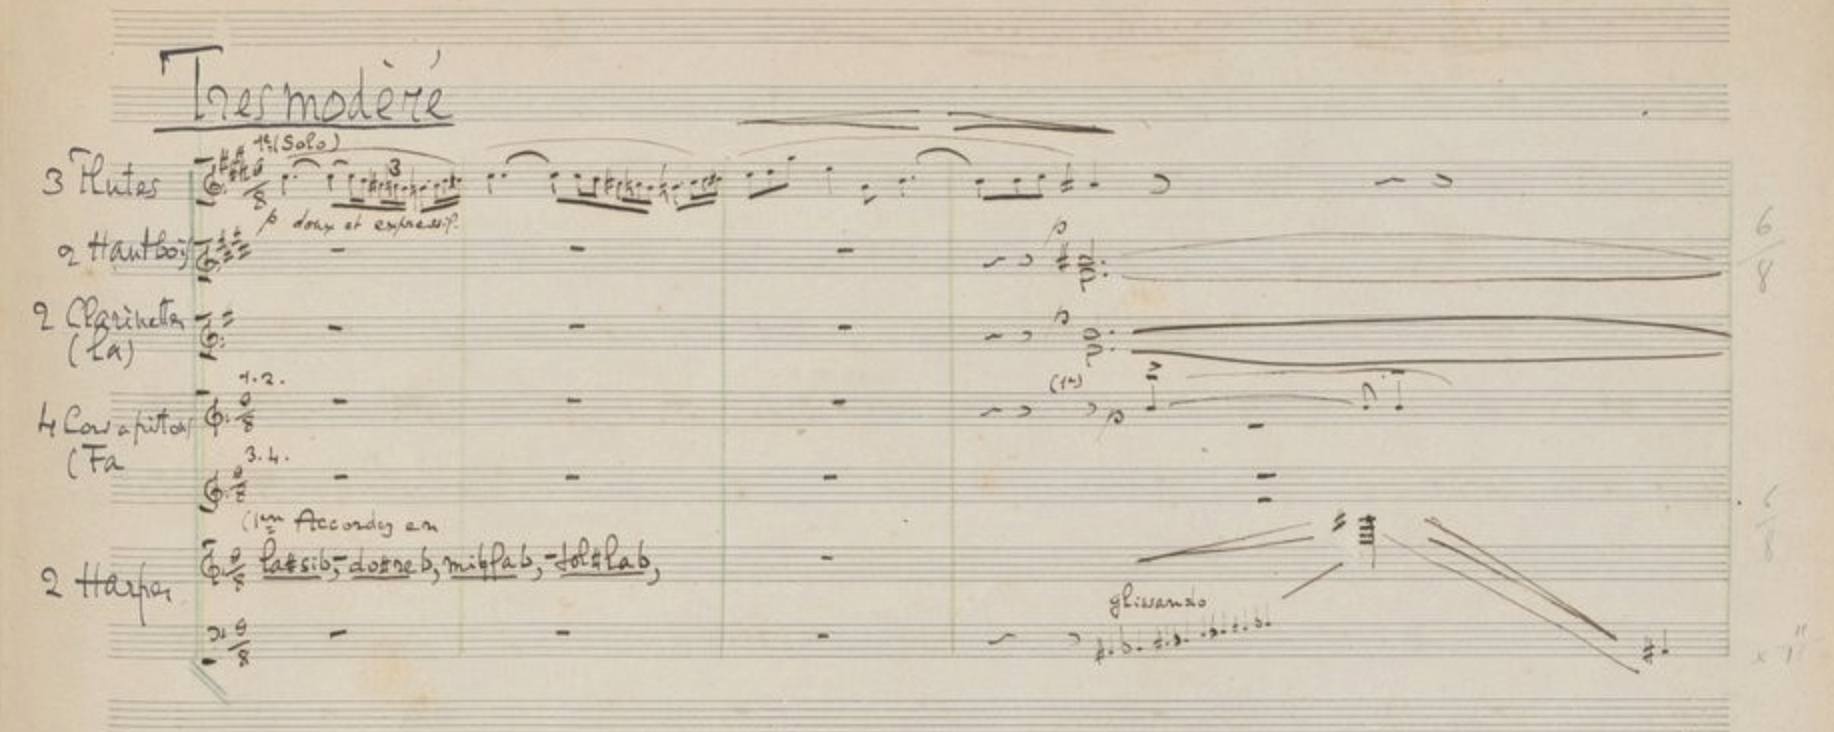
\includegraphics[width=1\textwidth]{illustrations/btv1b55001035h-f9.png}
    \caption{Extrait du \textit{Prélude \enquote{à l'après-midi d'un Faune}}, Claude Debussy, 1892-1894, manuscrit autographe, \url{https://gallica.bnf.fr/ark:/12148/btv1b55001035h/f9}.}
    \label{fig:btv1b55001035h-f9}
\end{figure}

Nous prendrons pour cas d'étude un extrait de la collection des manuscrits de partitions de piano attribués au compositeur Claude Debussy (1862 - 1918) \cite{barraque_debussy_1994}, conservés à la BnF et numérisés sur Gallica (fig. \ref{fig:btv1b55001035h-f9}). Contrairement aux partitions imprimées, ces sources présentent une hétérogénéité graphique s'écartant des standards de la \textit{Common Western Music Notation}\footnote{Système d'écriture occidental en vigueur depuis le \textsc{XVIII}e siècle, sur lequel nous nous concentrerons.} (CWMN) au profit de pratiques idiosyncratiques. Le document n'est plus un simple support de contenu musical abstrait, mais le témoin matériel d'un processus créatif (ratures, hésitations, annotations), mettant à l'épreuve les formats actuels face aux variabilités d'une source. 

\section{Travaux existants}

L'adéquation des formats d'encodage de la musique à la transcription automatique reste peu explorée, alors qu'elle définit la nature des informations extraites par les systèmes d'OMR. García-Iasci, Rizo et Calvo-Zaragoza \cite{garcia-iasci_evaluating_2025} et Castellanos, Gallego et Fujinaga \cite{castellanos_deep_2025} identifient la MEI, MusicXML et Humdrum **kern comme les standards prédominants, et soulignent l'efficacité des interfaces de transcription comme MuReT \cite{rizo_design_2023} et Sibelius \cite{avid_technology_sibelius_2024} pour l'exportation de ces données.

Toutefois, cette multiplicité de formats témoigne d'une fragmentation du champ de recherche. \textcite{torras_unified_2024} insiste sur la nécessité d'adopter un standard commun pour lever les freins technologiques de l'OMR et propose le \textit{Music Tree Notation} (MTN). Ce format intermédiaire, basé sur une structure de graphe, vise à fédérer la communauté en définissant les objets qui doivent être ciblés par l'OMR, ouvrant ainsi la voie à la création raisonnée de nouveaux jeux de données permettant l'entraînement et une meilleure évaluation des modèles d'OMR. 

\begin{figure}[H]
    \centering
    \begin{subfigure}[c]{0.40\linewidth} % [c] pour centrer verticalement
        \centering
        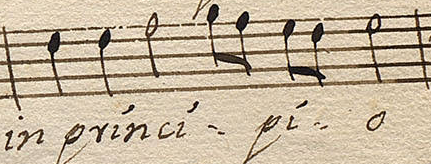
\includegraphics[width=\linewidth]{illustrations/pau-1.png}
        \caption{Extrait du Pau Llinás dataset \cite{baro_handwritten_2020}.}
        \label{subfig:pau}
    \end{subfigure}
    \hfill 
    \begin{subfigure}[c]{0.55\linewidth} % [c] ici aussi
        \centering
        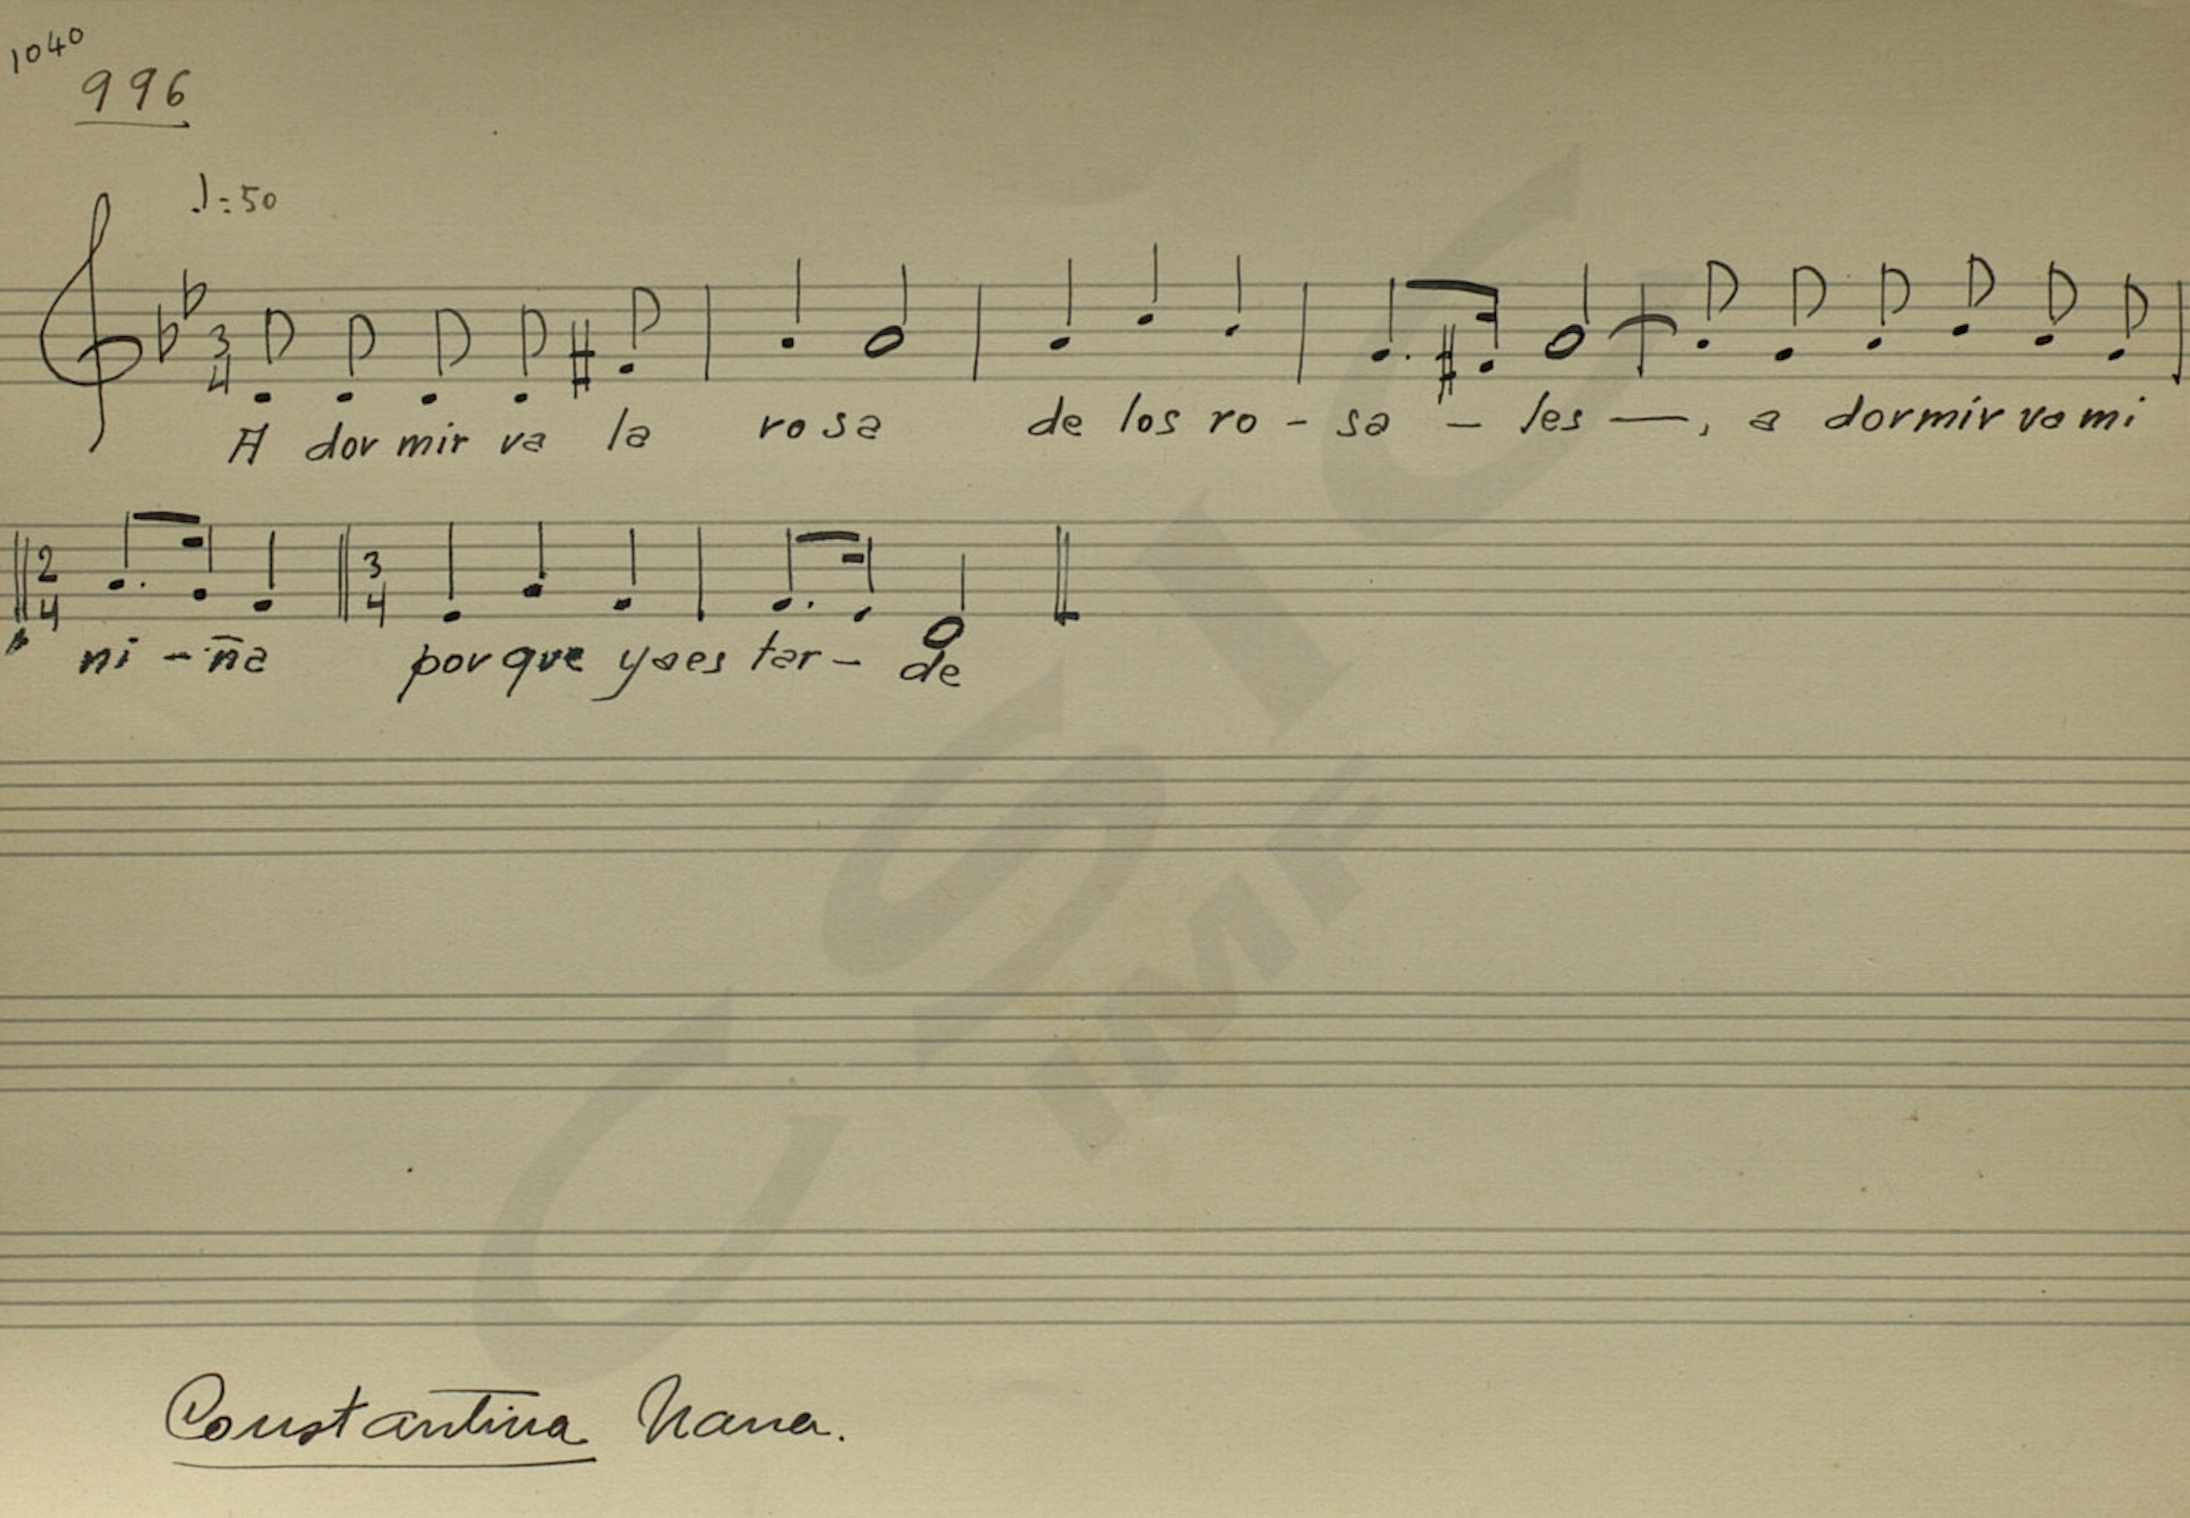
\includegraphics[width=\linewidth]{illustrations/m35_0996.png}
        \caption{Exemple d'un document provenant du FMT dataset : Óscar David Castillo Pérez, \textit{A dormir va la rosa}, Fondo de Música Tradicional IMF-CSIC, ed. E. Ros-Fábregas (consulté le 12/01/26), \url{https://musicatradicional.eu/piece/70690}.}
        \label{subfig:fmt}
    \end{subfigure}

    \caption{Exemples de jeux de données pour l'OMR manuscrit.}
    \label{fig:datasets-existant}
\end{figure}

\textcite{torras_unified_2024} souligne également que le manque de jeux de données larges et mutualisables demeure un obstacle majeur. Pour la CWMN manuscrite, et plus spécifiquement historique, les ressources exploitables sont rares, à l'exception du \textit{Pau Llinás dataset}\footnote{Le format d'annotation étant propriétaire, basé sur des chaînes de caractères, et dépourvu de coordonnées spatiales, cela limite fortement son interopérabilité.}~\cite{baro_handwritten_2020} (fig.~\ref{fig:datasets-existant}). Cette pénurie s'explique par le coût de l'expertise humaine et le caractère chronophage de l'annotation manuelle, poussant notamment une partie de la recherche vers la création de données synthétiques \cite{asbert_gan-based_2025, mayer_obstacles_2022}. 

Enfin, les rares corpus structurés en MusicXML ou MEI (SEILS \cite{parada-cabaleiro_seils_2017}, DoReMi \cite{shatri_doremi_2021}, PRIMuS \cite{calvo-zaragoza_camera-primus_2018}) s'avèrent inadaptés à notre étude car ils se concentrent soit sur la musique mensurale\footnote{La musique mensurale, ou notation mesurée, est un système de notation musicale utilisé en Europe entre le XIIIe et XVIIe siècles. Elle a fait l'objet de nombreuses études menées en OMR \cite{castellanos_neural_2020}.} \cite{calvo-zaragoza_end--end_2018}, soit sur des partitions numériques contemporaines. Si les jeux de données FMT-M et FMT-C \cite{ros-fabregas_codified_2021} semblent plus proches de notre objet d'étude, leur inaccessibilité actuelle nous empêche d'en évaluer la pertinence pour de l'OMR orienté vers la source.

\section{Quels formats disponibles pour un objectif de transcription automatique de partitions manuscrites ?}

\subsection{Les trois formats principaux de l'OMR}

La recherche actuelle repose sur trois formats dominants pour la CWMN : MusicXML, MEI et Humdrum **kern\footnote{Nous avons délibérément écarté certains formats de cette étude, comme Lilypond \cite{nienhuys_lilypond_2024}, PAEC \cite{rism_editorial_center_paec_2021} ou la ABC notation \cite{walshaw_abc_2011}, dont l'usage reste marginal dans les travaux actuels sur l'OMR. D'autres structures de représentation, telles que les graphes (MuNG) \cite{hajic_search_2017} n'ont pas été explorées pour cet article. Sans nous avancer davantage, un format tel que MuNG a comme principal défaut de n'être adapté qu'à la représentation de la sémantique du contenu musical.}. Si chacun permet de décrire le contenu musical sémantique, ils divergent par leurs priorités : l'échange et le rendu pour MusicXML, l'édition critique pour la MEI et l'analyse computationnelle pour Humdrum **kern.

Les formats MusicXML et MEI reposent sur le langage hiérarchique XML. MusicXML s'est imposé comme le standard d'échange entre logiciels d'édition (MuseScore \cite{musescore_bvba_musescore_2024}, Sibelius), intégrant la représentation du contenu musical et des instructions de mise en page nécessaires au rendu visuel d'une partition. Il ne permet pas nativement de lier le contenu à une source externe, comme pourrait le faire le format ALTO XML pour le texte \cite{alto_editorial_board_alto_2024}. À l'inverse, la MEI, conçue sur le modèle de la TEI \cite{tei_consortium_tei_2024}, est dédiée aux éditions\footnote{Voir, par exemple, la \href{https://dme.mozarteum.at/movi/}{Digital-Interactive Mozart Edition}, publiée par la International Mozarteum Foundation, Salzburg, ainsi que les autres projets listés sur le \href{https://music-encoding.org/community/projects-users.html}{site officiel de la MEI}, consultés le 12 janvier 2026.}. Elle autorise une description fine des phénomènes musicaux et un lien granulaire avec la source originale, mais sa grande flexibilité et sa verbosité la rendent complexe à exploiter pour de l'OMR.

Humdrum **kern propose une structure textuelle tabulaire. Sa concision facilite sa tokenisation, ce qui explique sa prédominance dans les modèles d'apprentissage profond récents \cite{rios-vila_sheet_2024, rios-vila_sheet_2024-1, cerveto-serrano_kernpy_2025}\footnote{Concernant la tokenisation des données d'entraînement pour l'OMR, \textcite{mayer_practical_2024} proposent une linéarisation du format MusicXML pour l'optimiser aux tâches d'apprentissage machine. Cette approche a permis d'introduire le format \textit{Linearized MusicXML} (LMX).}. Sa conception privilégie la sémantique musicale au détriment de la topographie documentaire, et, comme le souligne \textcite{torras_unified_2024}, il échoue à représenter la mise en page originale ou les éléments non structurels (groupements, nuances complexes), rendant impossible une restitution fidèle de la source manuscrite.

Nous considérons que deux conditions doivent être remplies pour qu'un format soit adapté à représenter une source dans le cadre d'une transcription basée sur une segmentation préalable : assurer l'ancrage spatial des objets à l'aide de coordonnées $(x, y)$ et permettre leur encodage graphique sans les contraintes d'une grammaire musicale normalisatrice et d'une simplification excessive. 

\subsection{Fidélité de la représentation de la source et ancrage spatial de la transcription}

Plutôt que l'édition scientifique, notre travail vise la création de vérités de terrain pour de l'apprentissage supervisé. En intégrant les phénomènes manuscrits et la matérialité du document, l'OMR pourrait ainsi devenir un levier pour l'histoire de la création musicale.

MusicXML, conçu pour garantir l'interopérabilité, l'échange de partitions structurées et leur reproduction (\textit{engraving}), ne permet pas nativement d'aligner les objets musicaux aux pixels d'une source. Cette caractéristique est pourtant stabilisée en ATR grâce aux formats ALTO et PAGE XML \cite{pletschacher_page_2010}, qui ancrent chaque caractère à une zone précise de l'image.

En ce qui concerne la représentation de la sémantique musicale, les schémas de MusicXML, Humdrum **kern et MEI sont suffisamment matures pour modéliser l'ensemble des objets sémantiques de la CWMN contemporaine : par exemple les notes et leurs différentes propriétés (durée, rythme, hauteur, etc.) ; ainsi que les ornements, les dynamiques, les clés, les barres de mesure, etc. Comme expliqué par \textcite{rettinghaus_pushing_2025}, le verrou n'est pas tant dans la richesse des schémas que dans l'incapacité des interfaces de transcription à exploiter pleinement ces structures. La question suivante est de savoir dans quelle mesure un format comme MusicXML peut représenter la matérialité de la source.

\section{De la note au signe : enjeux paléographiques de la création de vérités de terrain pour de l'OMR de partitions manuscrites} 

\subsection{Pour une approche graphématique de la transcription de la notation musicale}

L'OMR souffre également d'une absence de consensus sur la modélisation des objets à extraire. Comme l'indique \textcite{kiessling_transcription_2025}, la plupart des corpus de référence en ATR n'explicitent pas leur vocabulaire, rendant toute comparaison entre eux difficile. L'OMR ne fait pas exception à ce manque de transparence, comme le prouve l'hétérogénéité des classes entre les corpus de références \cite{castellanos_deep_2025}. À notre connaissance, seules deux tentatives de formalisation exhaustive existent : une première définissant 94 classes \cite{shatri_doremi_2021}, et une seconde où 88 sont dénombrées \cite{torras_unified_2024}.

La définition de ces objets soulève des problématiques musicologiques complexes qui dépassent le cadre de cet article et mériteraient une étude dédiée. Néanmoins, cette question est cruciale car elle conditionne notre capacité à représenter le contenu musical, et à s'accorder pour créer de nouvelles vérités de terrain interopérables. Comme l'explique \textcite{pinche_editing_2025}, la transcription est un acte de modélisation dont les choix techniques conditionnent les usages futurs de cet objet scientifique. Une telle approche suppose cependant l'existence de formats capables de porter cette modélisation. Il s'agit donc de déterminer la capacité de ces standards à représenter fidèlement la source originale et sa notation, au-delà de la seule abstraction du contenu musical.

\begin{figure}[H]
    \centering
    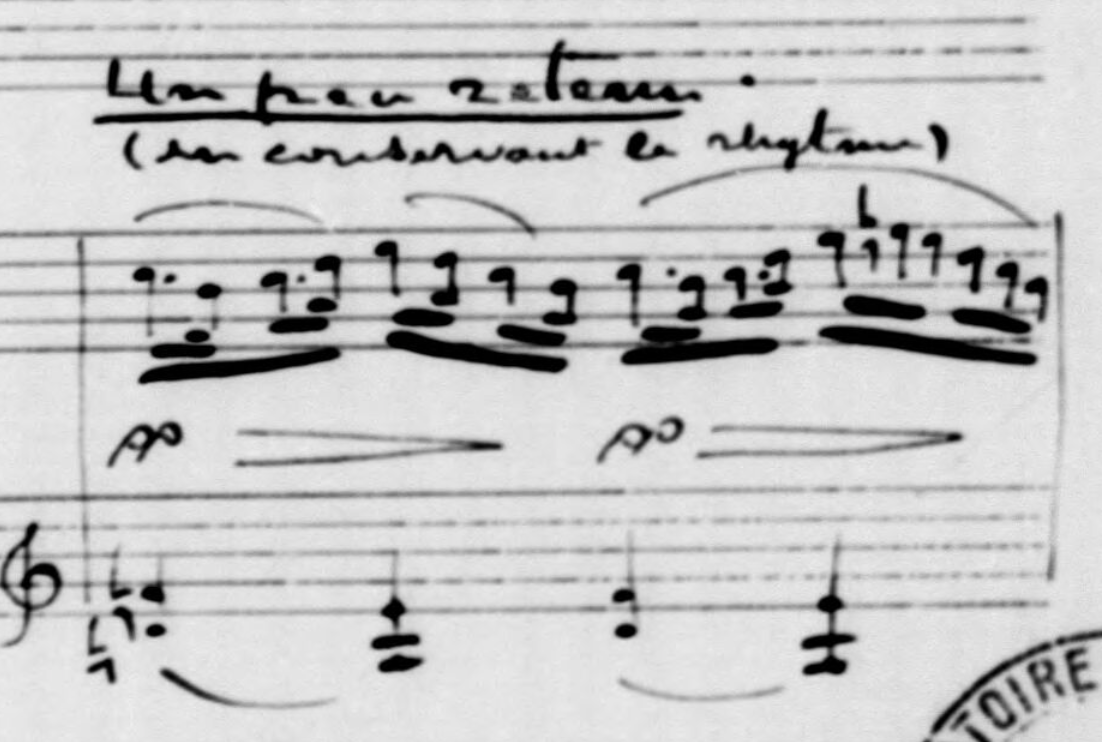
\includegraphics[width=0.4\linewidth]{illustrations/12148_btv1b100762337_f13.png}
    \caption{Extrait de \textit{Children's Corner}, Claude Debussy, non daté, manuscrit autographe, \url{https://gallica.bnf.fr/ark:/12148/btv1b100762337/f13}. Cette mesure présente des omissions dans les motifs rythmiques : absence de doubles croches pointées dans le motif du deuxième temps, similaire à celui du premier temps, et omissions de la notation des triolets dans le dernier temps.}
    \label{fig:12148_btv1b100762337_f13}
\end{figure}

S'appuyant sur les travaux de \textcite{pinche_editing_2025}, nous adoptons une approche graphématique pour la transcription de la CWMN historique, et l'appliquons à MusicXML. Contrairement à une transcription normalisée ou graphétique (décrivant chaque allographe), ce niveau se focalise, dans notre cas, sur l'orthographe musicale et la représentation des phénomènes matériels. Ce choix constitue le meilleur équilibre entre \enquote{rigueur formelle et faisabilité pratique et technique} \cite{pinche_editing_2025, kiessling_transcription_2025} : il harmonise les pratiques collaboratives, limite le nombre de classes à apprendre lors de l'entraînement d'un modèle et préserve l'intégrité visuelle de la source \cite{pinche_editing_2025, clerice_catmus_2024-1}.

Suivant les conclusions de \textcite{pinche_editing_2025, clerice_catmus_2024-1}, nous reconnaissons qu'une représentation parfaitement identique de la source n'est pas possible dans le cas d'une source musicale. Notre modèle doit reposer sur une simplification raisonnée. Ce choix évite au modèle de devoir internaliser des règles complexes de syntaxe musicale (ou de normalisation pour l'ATR \cite{kiessling_transcription_2025}) qui peuvent être source d'hallucinations \cite{clerice_paramhtrs_2026}. L'approche graphématique garantit une performance computationnelle tout en respectant l'intégrité de la source (fig. \ref{fig:12148_btv1b100762337_f13}, \ref{fig:normalise-graphematic.drawio-1}).

\begin{figure}[H]
    \centering
    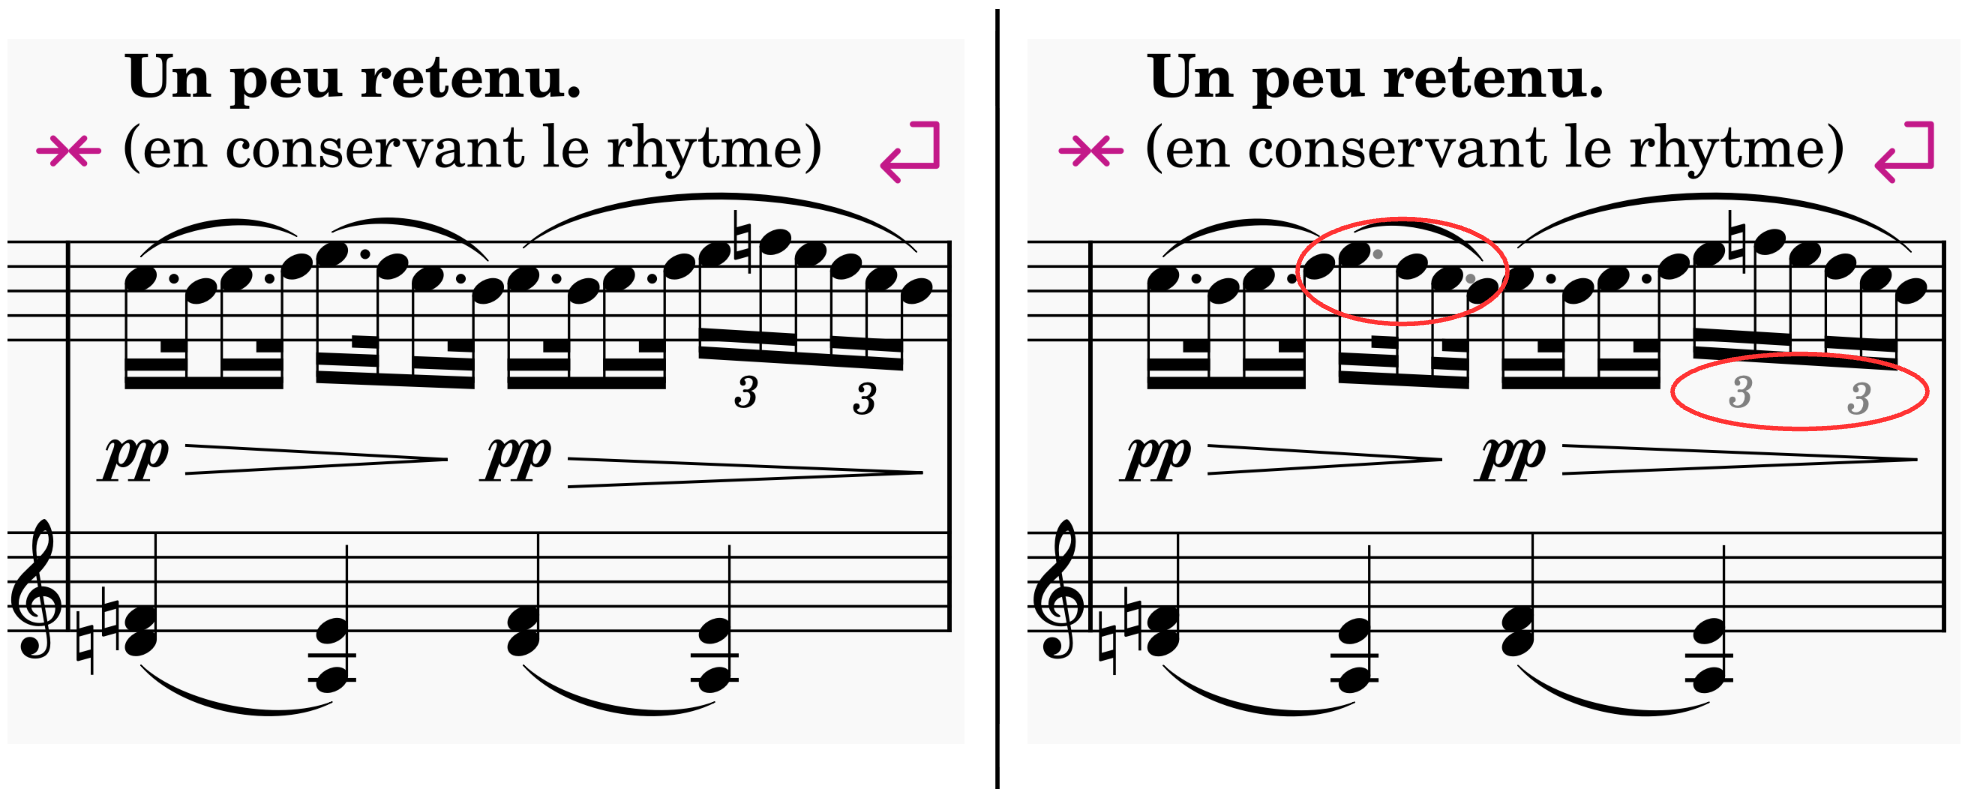
\includegraphics[width=0.9\linewidth]{illustrations/normalized-graphematic.drawio.png}
    \caption{Illustration d'une transcription de la fig. \ref{fig:12148_btv1b100762337_f13} avec MuseScore. À gauche, une transcription normalisée, où les indications rythmiques ont été corrigées. À droite, une transcription graphématique avec MuseScore. Nous avons utilisé l'outil \enquote{invisible} de MuseScore qui permet de cacher certains éléments graphiques (et qui apparaissent ici grisés), et qui seront indiqués lors de l'export en MusicXML en tant qu'attribut XML. Ils peuvent ainsi être supprimés en post-traitement, cassant ainsi la rythmique de la mesure, mais préservant son aspect visuel.}
    \label{fig:normalise-graphematic.drawio-1}
\end{figure}

\subsection{Les phénomènes non-standards comme obstacles à la représentation de la source : MusicXML face à la transcription graphématique}

Les manuscrits de partitions foisonnent de phénomènes « non-standards » : des éléments graphiques ou structurels s'écartant de la syntaxe normalisée pour s'inscrire dans une pratique manuscrite spécifique, à savoir des irrégularités de notation (rythmes implicites, omissions), d'artefacts physiques (ratures, annotations manuscrites) ou de contraintes de mise en page. Ces singularités révèlent une tension entre deux ontologies : l'approche sémantique centrée sur la logique musicale et ancrée dans la philosophie de MusicXML, et l'approche graphématique, centrée sur la morphologie des signes.

La gestion des indications textuelles illustre notamment cette limite. MusicXML traite le texte comme une métadonnée ancrée ponctuellement à l'échelle de la mesure, empêchant ainsi la représentation de son déploiement spatial, par exemple quand une indication s'étend sur plusieurs mesures ou systèmes. Faute de liens structurels entre le texte et la source, nous choisissons de limiter MusicXML aux symboles musicaux et aux symboles textuels de nature musicale. Les sources musicales présentent parfois des objets au statut hybride, principalement des indications de nuances et de dynamiques, où le signe textuel porte une instruction de jeu, et donc une information musicale. Si les indications de dynamique musicales conventionnelles ($p$, $f$) sont nativement gérées par MusicXML, les nuances idiosyncratiques du compositeur ne peuvent être représentées de façon standardisée (fig. \ref{fig:12148_btv1b55002573h_f9}). Afin de transcrire une source, cette approche impose donc une représentation binaire : une structuration MusicXML pour la donnée musicale et une modélisation tierce pour les éléments textuels. Cette fragmentation empêche une appréhension unitaire du document au sein d'un format unique.

\begin{figure}[H]
    \centering
    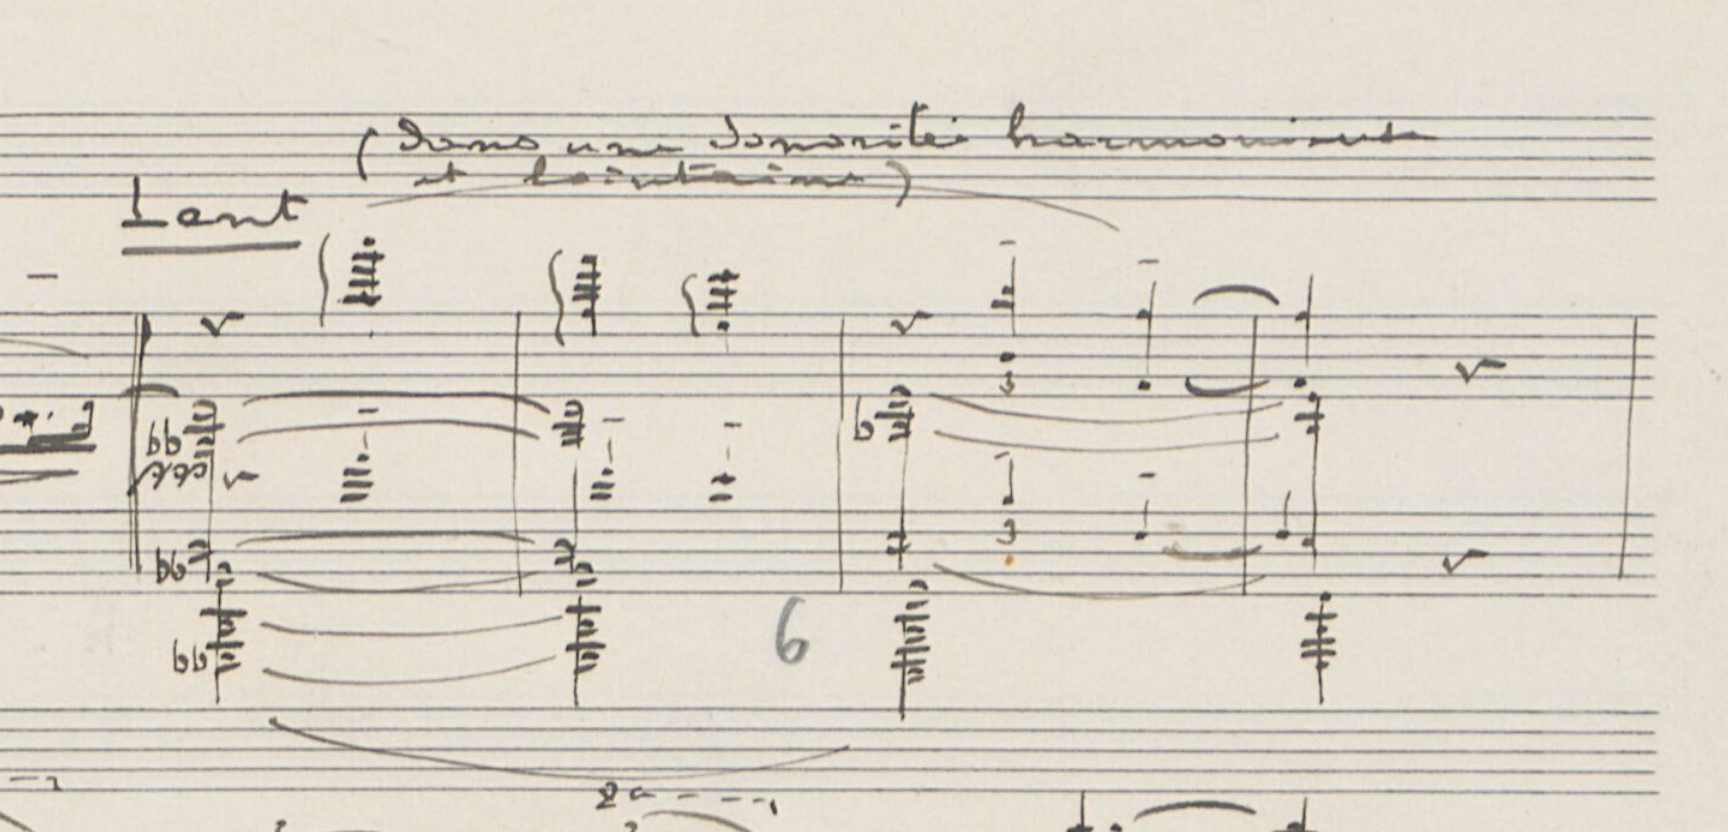
\includegraphics[width=0.8\linewidth]{illustrations/12148_btv1b55002573h_f9.png}
    \caption{Extrait des \textit{Reflets dans l'eau}, Claude Debussy, 1901-1905, manuscrit autographe, \url{https://gallica.bnf.fr/ark:/12148/btv1b55002573h/f9}. Au début de la première mesure de cet extrait, on observe un symbole de dynamique commun à l'ensemble de l'histoire de la CWMN : $ppp$, tandis qu'au-dessus des mesures, Debussy utilise une indication de tempo avec son propre vocabulaire : \enquote{Lent (dans une sonorité harmonieuse et lointaine)}. Le premier élément serait inclus dans notre proposition de transcription, tandis que le second relève des habitudes d'écriture de Debussy, et ne peut pas être représenté de façon normalisée avec MusicXML.}
    \label{fig:12148_btv1b55002573h_f9}
\end{figure}

Nous pouvons utiliser MusicXML pour représenter un semblant de structure en faisant appel à ses éléments de mise en page. Par exemple, lorsque couplé à une étape préliminaire d'analyse et de segmentation de systèmes \cite{castellanos_region-based_2022}, nous pouvons sommairement représenter leur structure interne grâce aux sauts de ligne. Or, la fidélité graphique exige parfois de représenter des cas plus complexes, comme celui de mesures scindées entre deux systèmes (fig. \ref{fig:12148_btv1b108610504_f43}). Dans ce cas, nous privilégions la représentation documentaire en fragmentant l'unité logique en deux entités distinctes, contrairement au schéma de MusicXML qui impose qu'une mesure soit une unité logique close. La cohérence musicale est ainsi sacrifiée au profit de la structure physique. Cela transforme l'usage du format où la hiérarchie sémantique s'efface devant la topographie du manuscrit.

\begin{figure}[H]
    \centering
    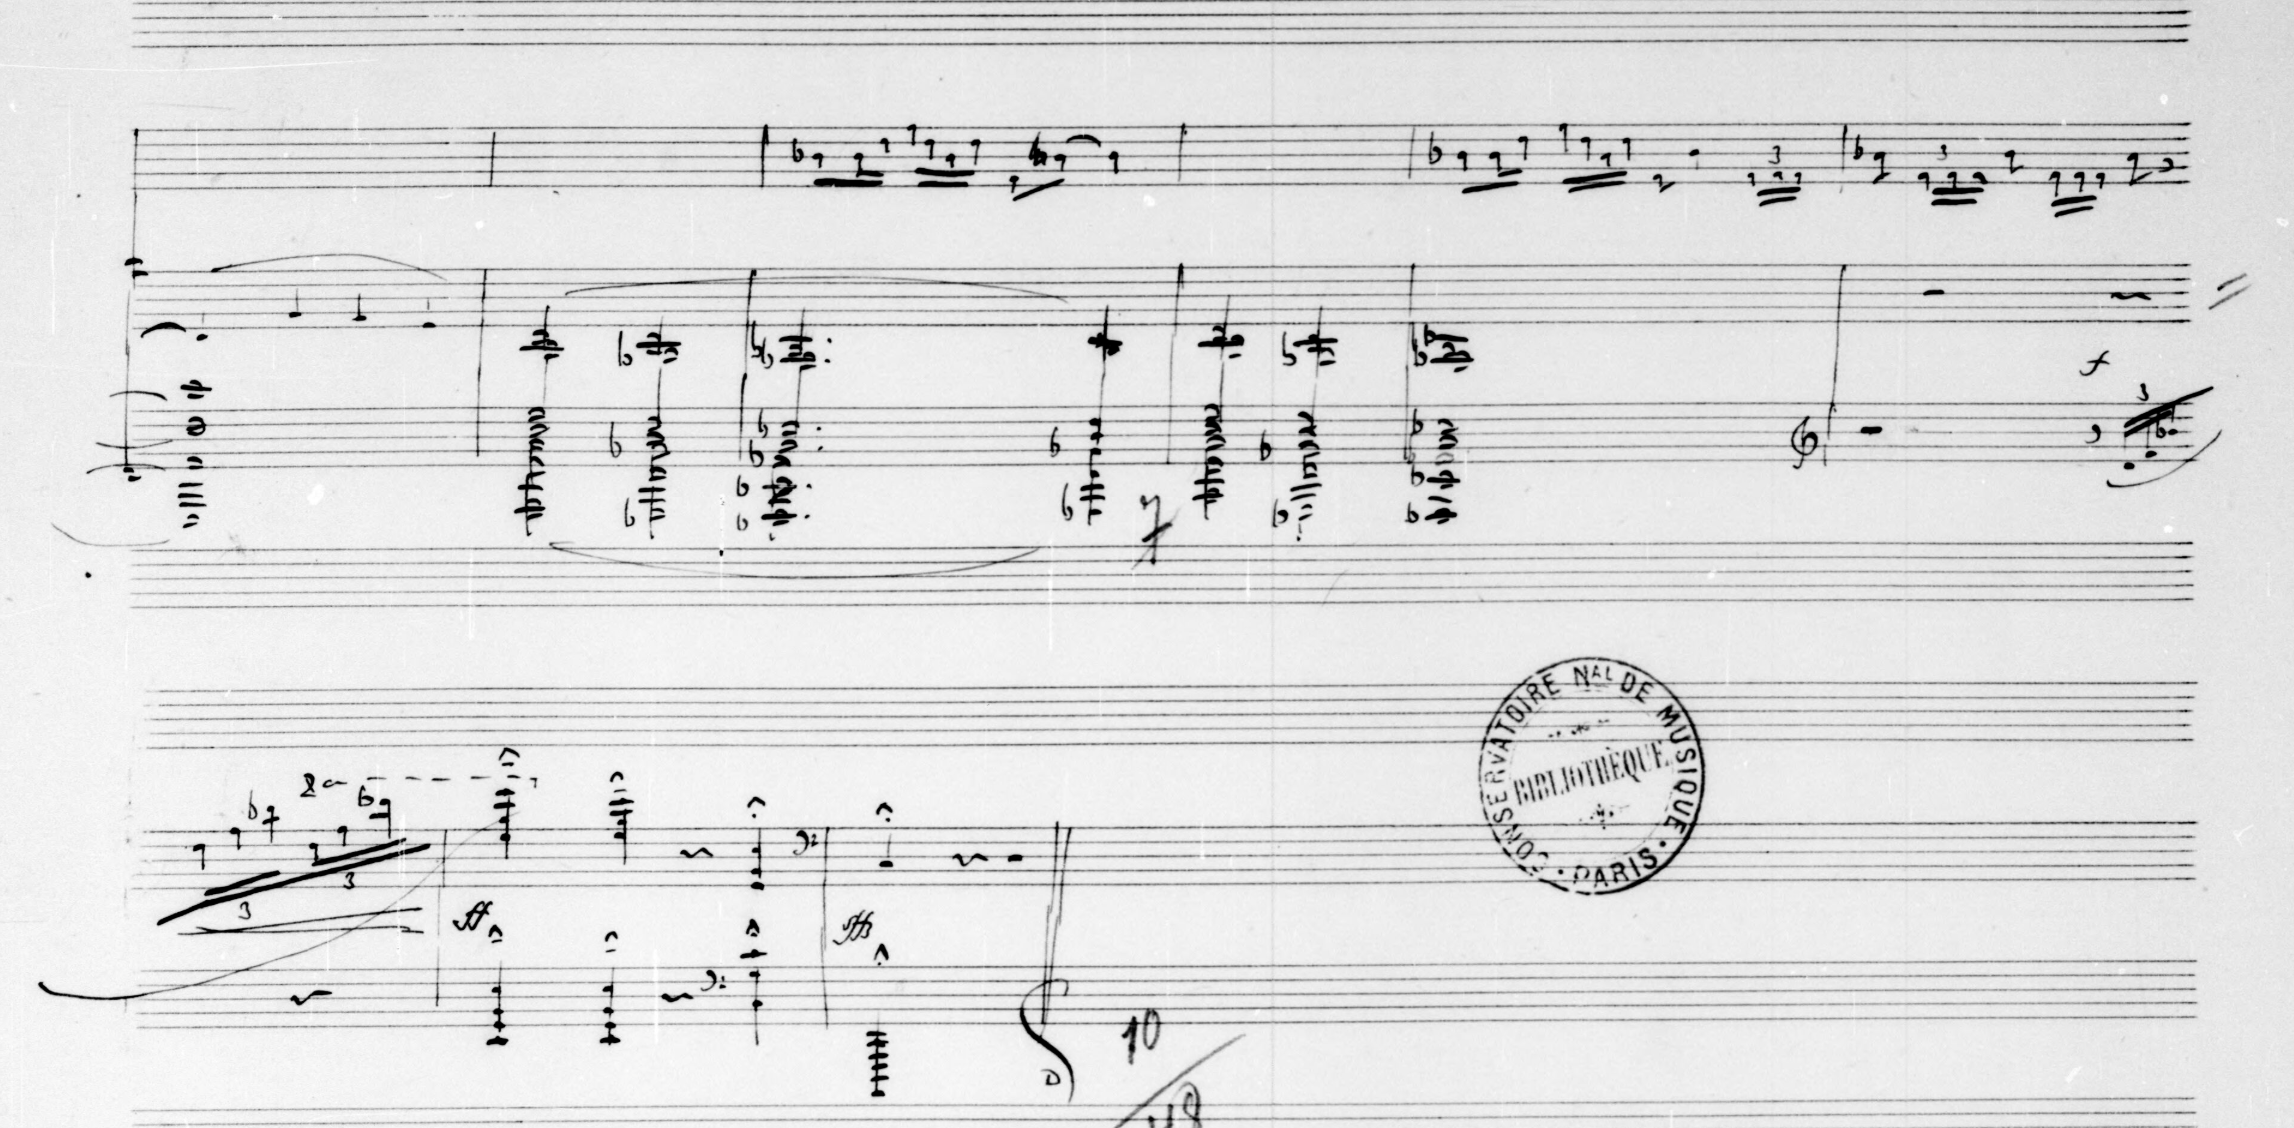
\includegraphics[width=0.8\linewidth]{illustrations/12148_btv1b108610504_f43.png}
    \caption{Extrait de \textit{La Boîte à joujoux, ballet en 3 tableaux, piano seul}, Claude Debussy, non daté, manuscrit autographe, \url{https://gallica.bnf.fr/ark:/12148/btv1b108610504/f43}. Exemple d'une mesure scindée entre deux systèmes.}
    \label{fig:12148_btv1b108610504_f43}
\end{figure}

Enfin, MusicXML ne peut représenter nativement les ratures, les repentirs ou les symboles ambigus, comme par exemple ceux utilisés pour représenter des répétitions non-standardisées (fig. \ref{fig:12148_btv1b10073993b_f2}, \ref{fig:12148_btv1b10073993b_f2-detail}, \ref{fig:12148_btv1b10860171f_f10}, \ref{fig:12148_btv1b52000863t_f17}). Leur intégration suppose un détournement du schéma original par l'usage de caractères de substitution. 

\begin{figure}[H]
    \centering
    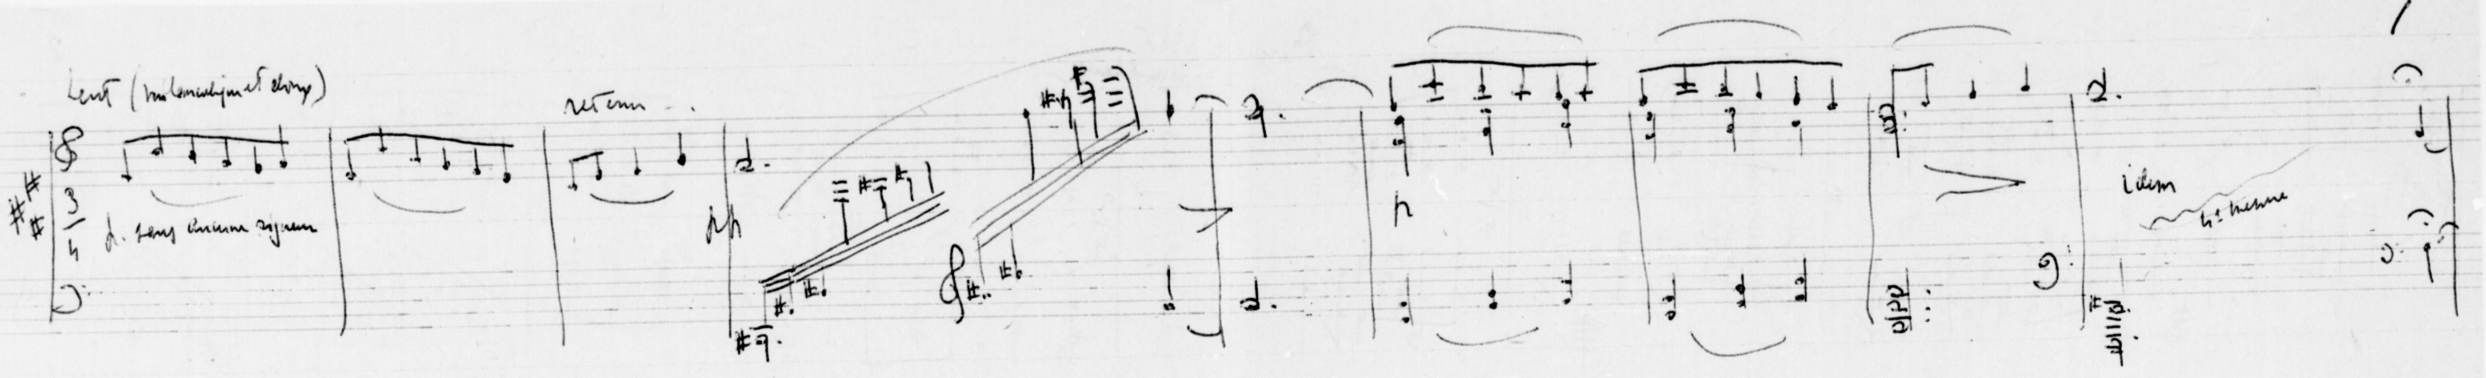
\includegraphics[width=1\linewidth]{illustrations/12148_btv1b10073993b_f2.png}
    \caption{Extrait des \textit{Images oubliées, n° 1, pour piano}, Claude Debussy, non daté, manuscrit autographe, \url{https://gallica.bnf.fr/ark:/12148/btv1b10073993b/f4.item}.}
    \label{fig:12148_btv1b10073993b_f2}
\end{figure}

\begin{figure}[H]
    \centering
    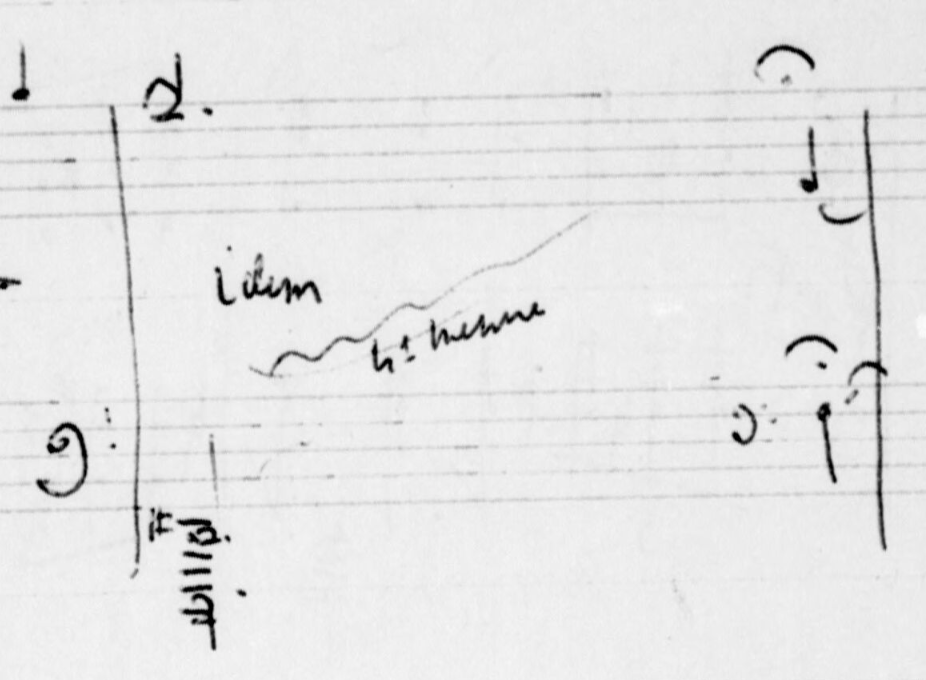
\includegraphics[width=0.4\linewidth]{illustrations/12148_btv1b10073993b_f2-detail.png}
    \caption{Détail de la fig. \ref{fig:12148_btv1b10073993b_f2} Marque de répétition inhabituelle, ici Debussy indique la répétition d'un motif isolé présent dans la quatrième mesure d'un système. Dans ladite mesure illustrée ici, le premier temps et le dernier temps sont cependant différents.}
    \label{fig:12148_btv1b10073993b_f2-detail}
\end{figure}

\begin{figure}[H]
    \centering
    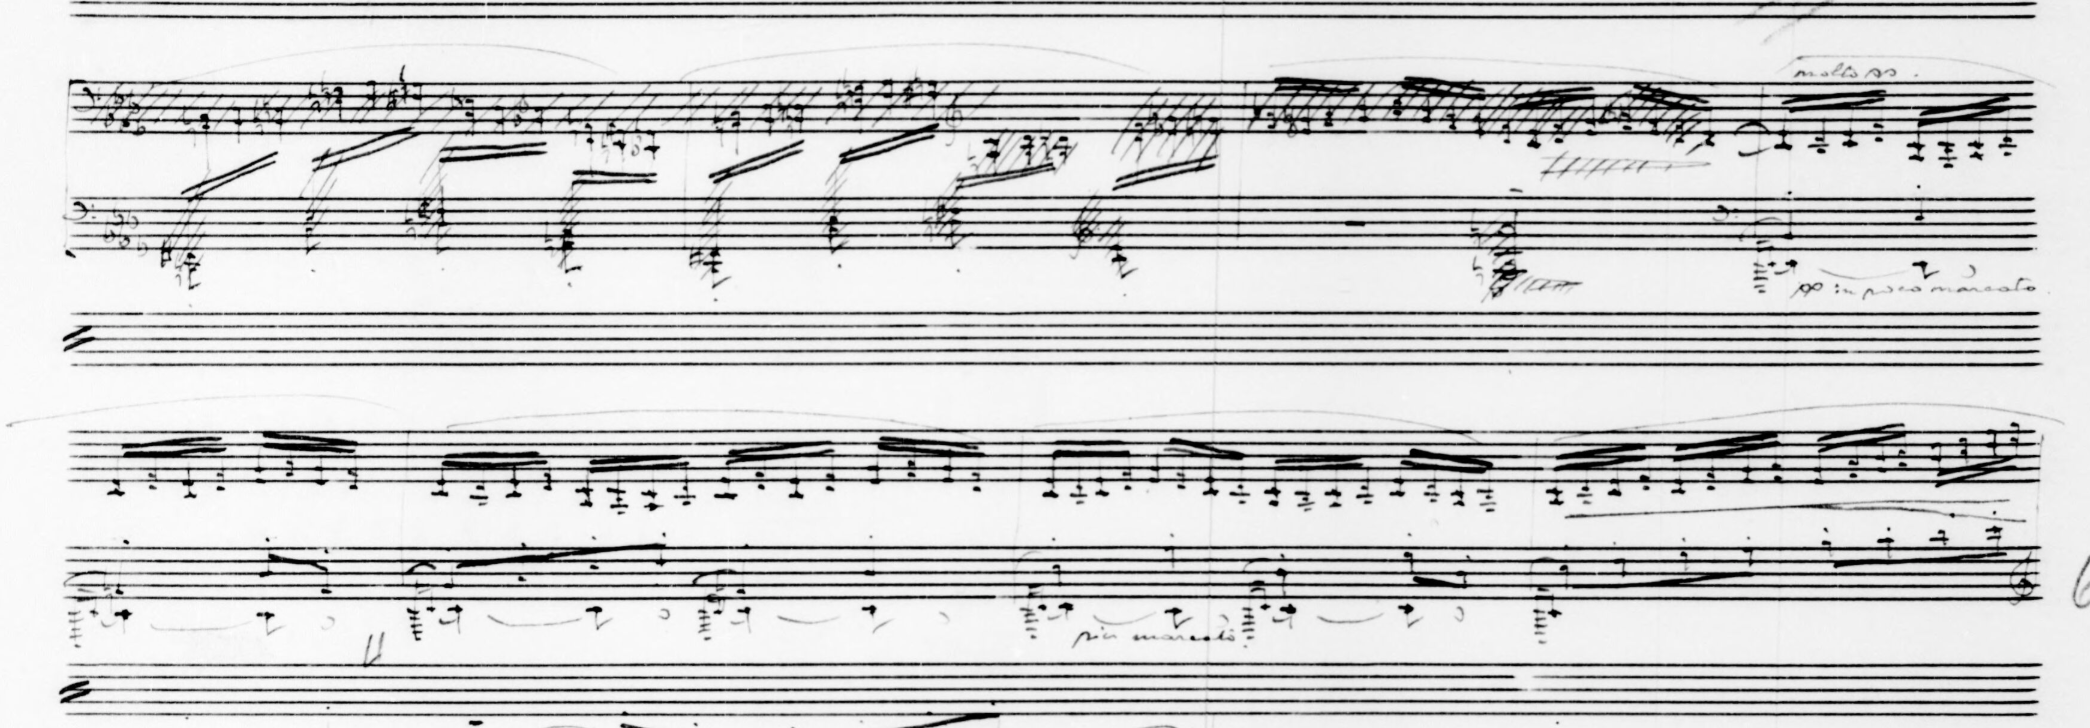
\includegraphics[width=1\linewidth]{illustrations/12148_btv1b10860171f_f10.png}
    \caption{Extrait de \textit{Douze études pour le piano, livres I et II}, Claude Debussy, non daté, manuscrit autographe, \url{https://gallica.bnf.fr/ark:/12148/btv1b10860171f/f10.item}. On y observe de nombreuses ratures : mesures complètes, notes, dynamiques.}
    \label{fig:12148_btv1b10860171f_f10}
\end{figure}

\begin{figure}[H]
    \centering
    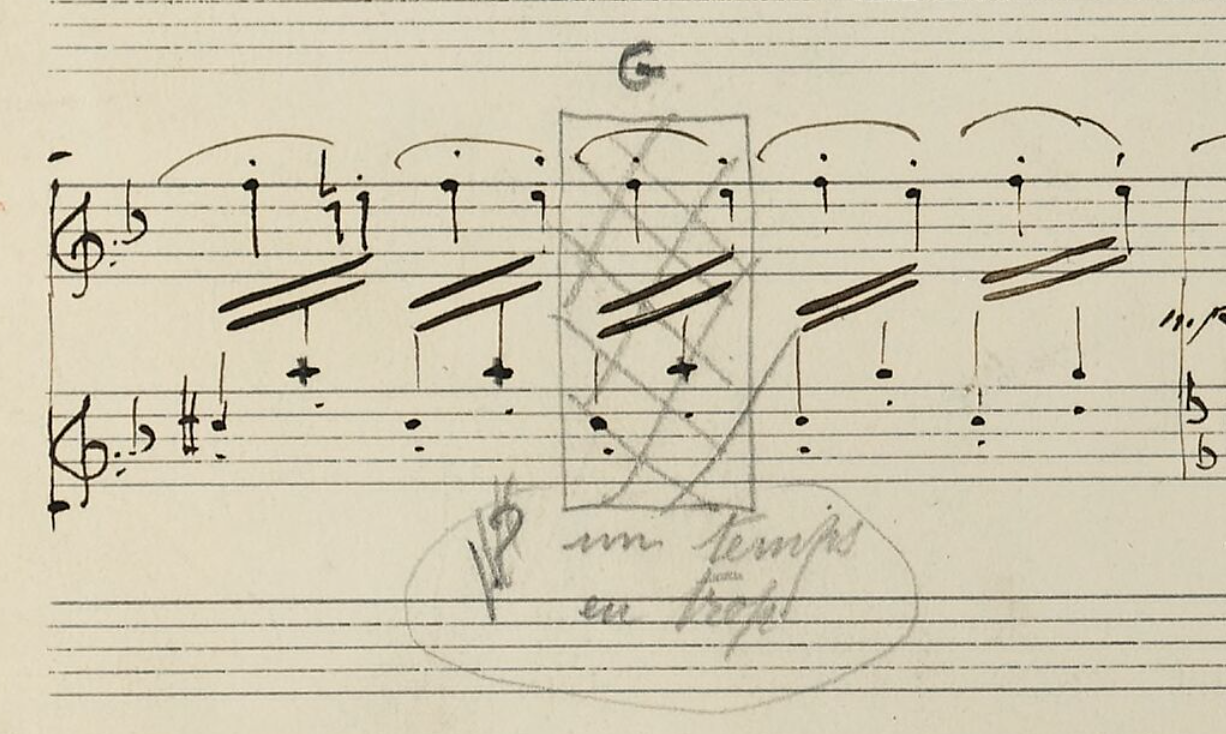
\includegraphics[width=0.5\linewidth]{illustrations/12148_btv1b52000863t_f17.png}
    \caption{Extrait de \textit{Children's Corner}, Claude Debussy, 1908, manuscrit autographe, \url{https://gallica.bnf.fr/ark:/12148/btv1b52000863t/f17}. Lors de l'édition, un motif musical a été raturé car étant un temps en trop dans la mesure.}
    \label{fig:12148_btv1b52000863t_f17}
\end{figure}

Ces détournements nous conduisent à définir un MusicXML \enquote{structurel}. Ce modèle de données n'est pas une partition fonctionnelle destinée à être affichée (\textit{engraving}), mais une représentation où la structure matérielle du document prime sur sa validité théorique. En neutralisant les contraintes sémantiques les plus rigides au profit d'une vérité terrain fidèle à la source, ce MusicXML détourné devient un pivot pour l'entraînement de modèles capables de capturer son hétérogénéité.

\section{Conclusion}

L'état des lieux dressé révèle une forme de dette technique et ses conséquences scientifiques pour l'OMR. Entre le réductionnisme de Humdrum **kern et l'exhaustivité éditoriale de la MEI, MusicXML s'impose comme le pivot le plus pragmatique. Sa capacité à représenter la sémantique musicale et une mise en page sommaire, ainsi que son interopérabilité avec des éditeurs \textit{open-source} tels que MuseScore en font un outil de production de données accessible, malgré son incapacité native à aligner le contenu musical sur la topographie de la source, qui échappe à la pure sémantique musicale.\footnote{Notre choix a été motivé par l'absence d'accès public à l'interface MuRet, pourtant optimisée pour la recherche en OMR \cite{garcia-iasci_evaluating_2025} et pour la transcription de sources musicales historiques \cite{rizo_design_2023}. Nous avons également écarté les solutions propriétaires (PhotoScore, Sibelius). MuseScore est un logiciel \textit{open-source}, il offre notamment une compatibilité croissante avec MusicXML grâce à son développement continu \cite{rettinghaus_pushing_2025}.}  

L'OMR orienté sources historiques semble souffrir d'un déficit d'infrastructure comparativement à l'ATR. Ce domaine a connu un saut qualitatif, porté non seulement par un progrès technologique, mais aussi par une profonde réflexion épistémologique sur ses standards. L'ATR offre à ce titre un miroir instructif : l'adoption généralisée du format ALTO XML pour l'échange de vérités de terrain, le développement de moteurs agnostiques comme Kraken intégrés dans des interfaces collaboratives telles qu'eScriptorium \cite{kiessling_kraken_2025, stokes_escriptorium_2021}, ont transformé la technologie en une véritable infrastructure de recherche. À l'image des initiatives pour la standardisation des \textit{guidelines} et le partage des vérités de terrain \cite{clerice_catmus_2024-1, chague_htr-united_2022}, l'OMR historique doit désormais stabiliser ses propres normes pour sortir de l'isolement des corpus spécifiques. En outre, la robustesse de MusicXML et celle de notre proposition graphématique demandent désormais à être confrontées à des structures de partition plus denses et plus complexes, comme des partitions d'orchestre.

En conclusion, l'avancement de l'OMR pour les sources historiques ne dépend pas seulement de la puissance des modèles, mais d'un accord collectif sur trois éléments : 
\begin{enumerate} 
    \item \textbf{Une interface permettant le couplage partition-image} pour garantir un alignement strict entre le pixel et l'annotation ; 
    \item \textbf{Un format d'encodage hybride} permettant une annotation granulaire, de la portée jusqu'à la page, inspiré d'ALTO XML ; 
    \item \textbf{La définition de \textit{guidelines} communes}, capables de résoudre les ambiguïtés de la CWMN face aux idiosyncrasies des manuscrits. 
\end{enumerate}

Comme le démontre \textcite{kiessling_transcription_2025}, si les modèles de transcription actuels affichent des performances satisfaisantes, leur fiabilité sur des données historiques reste limitée par la variabilité des sources et le manque de jeux de données de test représentatifs. La convergence vers des standards de représentation et une ontologie commune des signes musicaux, ainsi que vers des normes de transcription partagées, constitue ainsi les prérequis indispensables au développement d'un OMR robuste historique orienté sur la source.

% \section*{Remerciements}

% \section*{Financements}

% Imprime la bibliographie à la fin. Gardez cette ligne après le texte principal de votre article et avant une annexe.
\printbibliography

\end{document}

